% =====================================================================
% AI Academy -- National AI Center
% Software Engineering Final Project -- Presentation Deck
%
% Team: Byte Bite  |  Topic: 2 -- AI Food Analyzer
% =====================================================================

\PassOptionsToPackage{dvipsnames}{xcolor}
\documentclass[aspectratio=169,11pt]{beamer}

% ===== CONFIGURATION =================================================
\newcommand{\teamname}{Byte Bite}
\newcommand{\topicchoice}{Topic 2 --- AI Food Analyzer}
\newcommand{\memberone}{Aysel Mamedova}
\newcommand{\membertwo}{G\"{u}lnur M\k{a}mm\k{a}dova}
\newcommand{\memberthree}{\c{S}\k{a}mistan H\"{u}seynov}
\newcommand{\memberfour}{R\k{a}him\k{a} K\k{a}rimova}
\newcommand{\repolink}{github.com/AMammedova/food-analyzer-byte-bite}

\newcommand{\coursecode}{AI-ENG-110}
\newcommand{\coursename}{Software Engineering}
\newcommand{\institution}{AI Academy, National AI Center}
\newcommand{\semester}{Spring 2026}

% ===== PACKAGES ======================================================
\usepackage[T1]{fontenc}
\usepackage[utf8]{inputenc}
\usepackage{xcolor}
\usepackage{tabularx}
\usepackage{booktabs}
\usepackage{listings}
\usepackage{tikz}
\usetikzlibrary{shapes.geometric,arrows.meta,positioning,fit,backgrounds}

% ===== BEAMER THEME ==================================================
\usetheme{default}
\usefonttheme{professionalfonts}
\setbeamertemplate{navigation symbols}{}

\definecolor{accent}{HTML}{0B3D91}
\definecolor{soft}{HTML}{F2F4F8}
\definecolor{ok}{HTML}{166534}
\definecolor{warn}{HTML}{8B0000}

\setbeamercolor{title}{fg=accent}
\setbeamercolor{frametitle}{fg=accent}
\setbeamercolor{itemize item}{fg=accent}
\setbeamercolor{itemize subitem}{fg=accent}
\setbeamercolor{enumerate item}{fg=accent}
\setbeamercolor{block title}{bg=accent,fg=white}
\setbeamercolor{block body}{bg=soft,fg=black}

\setbeamerfont{title}{size=\Large,series=\bfseries}
\setbeamerfont{frametitle}{size=\large,series=\bfseries}
\setbeamerfont{footline}{size=\tiny}

\setbeamertemplate{footline}{%
  \leavevmode%
  \hbox{\hspace*{2ex}\tiny\textit{\teamname{} -- \topicchoice{}}\hfill%
  \tiny\textit{\coursecode{} -- \semester{}}\hfill%
  \tiny\insertframenumber/\inserttotalframenumber\hspace*{2ex}}%
  \vskip1pt%
}

% ===== CODE STYLE ====================================================
\lstdefinestyle{pysmall}{
  language=Python,
  backgroundcolor=\color{soft},
  keywordstyle=\color{accent},
  basicstyle=\ttfamily\scriptsize,
  breaklines=true,
  frame=single,
  framerule=0.4pt,
  rulecolor=\color{black!30},
  numbers=none,
}
\lstdefinestyle{bash}{
  language=bash,
  backgroundcolor=\color{soft},
  basicstyle=\ttfamily\scriptsize,
  breaklines=true,
  frame=single,
  framerule=0.4pt,
  rulecolor=\color{black!30},
  numbers=none,
}

% =====================================================================
\begin{document}

% ========== SLIDE 1: TITLE ===========================================
{%
\setbeamertemplate{footline}{}
\begin{frame}[plain]
  \begin{center}
    \vspace{0.4cm}
    {\small \textsc{\institution}}\\[0.2em]
    {\small \textsc{\coursecode{} -- \coursename{} -- \semester{}}}\\[1em]
    \rule{0.7\textwidth}{0.6pt}\\[0.4em]
    {\Huge\bfseries\color{accent} AI Food Analyzer}\\[0.3em]
    {\large\itshape Photo $\to$ Ingredients $\to$ Nutrition Facts}\\[0.4em]
    \rule{0.7\textwidth}{0.6pt}\\[0.8em]
    {\large\bfseries \teamname}\\[0.5em]
    {\small
      \memberone\enspace\textbullet\enspace
      \membertwo\enspace\textbullet\enspace
      \memberthree\enspace\textbullet\enspace
      \memberfour
    }\\[0.8cm]
    {\footnotesize\itshape Final Project Defense --- May 2026}\\[0.3em]
    {\footnotesize\texttt{\repolink}}
  \end{center}
\end{frame}
}

% ========== SLIDE 2: PROBLEM =========================================
\begin{frame}{The Problem}

  \begin{block}{What the system does}
    A user uploads a meal photo $\to$ the system identifies ingredients with portion sizes,
    queries USDA for nutrition data, and returns calories + macronutrients in under 2 seconds.
  \end{block}

  \vspace{0.4em}
  \begin{columns}[T,onlytextwidth]
  \column{0.46\textwidth}
    \textbf{Input}
    \begin{itemize}\setlength\itemsep{0.2em}
      \item Meal photo (JPEG / PNG, $\le$5\,MB)
      \item Validated at magic-byte level
    \end{itemize}
    \vspace{0.5em}
    \textbf{Entry points}
    \begin{itemize}\setlength\itemsep{0.2em}
      \item \texttt{POST /analyze} (HTTP API)
      \item \texttt{GET /} \enspace(web UI)
      \item \texttt{python -m foodanalyzer analyze} (CLI)
    \end{itemize}

  \column{0.50\textwidth}
    \textbf{Output}
    \begin{itemize}\setlength\itemsep{0.2em}
      \item Per-ingredient: name, grams, kcal, protein, carbs, fat
      \item Totals row
      \item Analysis saved to PostgreSQL
      \item History via \texttt{GET /history}
    \end{itemize}
  \end{columns}

\end{frame}

% ========== SLIDE 3: ARCHITECTURE ====================================
\begin{frame}{Architecture}

  \begin{columns}[T,onlytextwidth]
  \column{0.52\textwidth}
  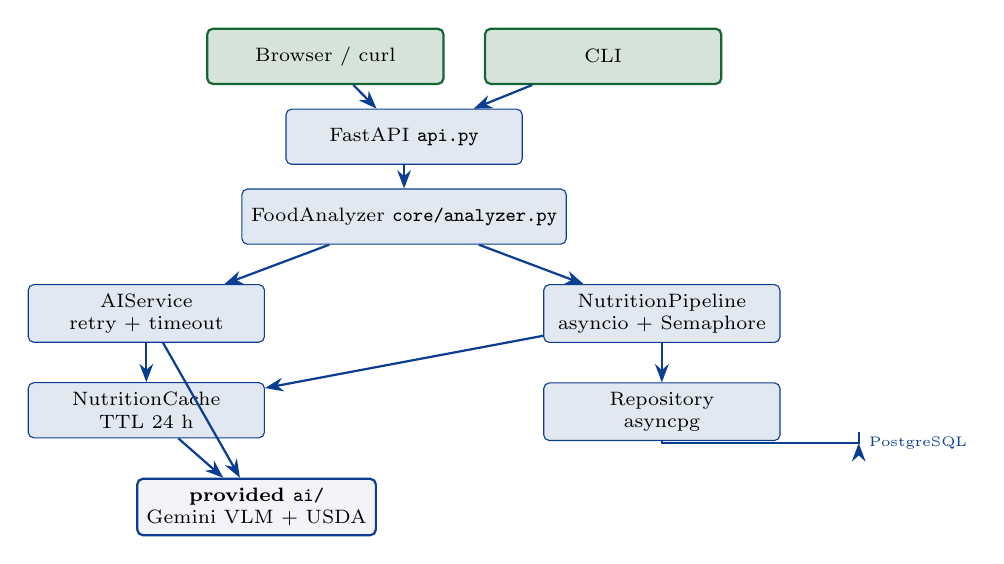
\begin{tikzpicture}[
    node distance=3mm and 4mm,
    box/.style={draw,rounded corners=2pt,minimum width=3cm,minimum height=0.7cm,
                align=center,font=\scriptsize},
    aibox/.style={box,fill=soft,draw=accent,thick},
    sebox/.style={box,fill=accent!12,draw=accent},
    entry/.style={box,fill=ok!18,draw=ok,thick},
    arrow/.style={-Stealth,thick,color=accent}
  ]
    \node[entry] (ui)  {Browser / curl};
    \node[entry,right=5mm of ui] (cli) {CLI};

    \node[sebox,below=of ui,xshift=1cm] (api) {FastAPI \texttt{api.py}};

    \node[sebox,below=of api] (core) {FoodAnalyzer \texttt{core/analyzer.py}};

    \node[sebox,below left=5mm and -3mm of core]  (svc)  {AIService\\retry + timeout};
    \node[sebox,below right=5mm and -3mm of core] (pip)  {NutritionPipeline\\asyncio + Semaphore};

    \node[sebox,below=5mm of svc]  (cache) {NutritionCache\\TTL 24 h};
    \node[sebox,below=5mm of pip]  (repo)  {Repository\\asyncpg};

    \node[aibox,below=5mm of cache,xshift=1.4cm] (ai) {\textbf{provided \texttt{ai/}}\\Gemini VLM + USDA};

    \draw[arrow] (ui)   -- (api);
    \draw[arrow] (cli)  -- (api);
    \draw[arrow] (api)  -- (core);
    \draw[arrow] (core) -- (svc);
    \draw[arrow] (core) -- (pip);
    \draw[arrow] (svc)  -- (cache);
    \draw[arrow] (pip)  -- (cache);
    \draw[arrow] (pip)  -- (repo);
    \draw[arrow] (svc)  -- (ai);
    \draw[arrow] (cache)-- (ai);
    \draw[arrow] (repo) |- ++(0,-0.4) -| ++(2.5,0) node[right,font=\tiny]{PostgreSQL};
  \end{tikzpicture}

  \column{0.45\textwidth}
  \vspace{0.3em}
  \textbf{Key boundary:} provided \texttt{ai/} is an external dependency --- we wrap it, never modify it.

  \vspace{0.6em}
  \textbf{Our SE layer adds:}
  \begin{itemize}\setlength\itemsep{0.3em}
    \item Retry + timeout (\texttt{tenacity})
    \item TTL cache (\texttt{asyncio.Lock})
    \item Concurrent fan-out (\texttt{asyncio.gather})
    \item Typed config (\texttt{pydantic-settings})
    \item Structured logging
    \item PostgreSQL persistence
    \item 158 offline tests
  \end{itemize}
  \end{columns}

\end{frame}

% ========== SLIDE 4: DESIGN DECISIONS ================================
\begin{frame}{Three Design Decisions We Can Defend}

  \begin{enumerate}\setlength\itemsep{0.7em}
    \item \textbf{Composition over inheritance in \texttt{FoodAnalyzer}}\\
      \texttt{FoodAnalyzer} receives \texttt{AIService} and \texttt{NutritionPipeline} as constructor args.\\
      \textit{Why:} the analyzer \emph{uses} these services, not specialises them ---
      dependency injection makes unit-testing trivial (swap in fakes, no monkey-patching).

    \item \textbf{asyncio over threading for USDA fan-out}\\
      USDA lookups are I/O-bound (network RTT $\sim$500\,ms each).\\
      \textit{Why:} \texttt{asyncio} gives cooperative concurrency with zero OS-thread overhead;
      \texttt{ProcessPoolExecutor} would be right only for CPU-bound work.

    \item \textbf{pydantic-settings for typed configuration}\\
      One \texttt{Settings} class reads from \texttt{.env}, validates types, and fails fast at startup.\\
      \textit{Why:} eliminates scattered \texttt{os.getenv()} calls; type errors surface before the first request.
  \end{enumerate}

\end{frame}

% ========== SLIDE 5: CONCURRENCY =====================================
\begin{frame}{Concurrency: the Benchmark}

  \textbf{How it works:} \texttt{NutritionPipeline.fetch\_all()} fans out $N$ USDA lookups
  via \texttt{asyncio.gather}, bounded by \texttt{Semaphore(MAX\_PARALLEL=10)}.

  \vspace{0.5em}
  \begin{center}\small
  \begin{tabular}{lcccr}
    \toprule
    \textbf{Workload} & $N$ & \textbf{Sequential (s)} & \textbf{Concurrent (s)} & \textbf{Speedup} \\
    \midrule
    Nutrition lookups & 3 & 1.51 & 0.50 & 3.0$\times$ \\
    Nutrition lookups & 5 & 2.50 & 0.53 & \textbf{4.8$\times$} \\
    Nutrition lookups & 7 & 3.51 & 0.52 & 6.7$\times$ \\
    \bottomrule
  \end{tabular}
  \end{center}

  \vspace{0.3em}
  {\footnotesize Conditions: simulated 0.5\,s USDA latency, caches cleared, Python 3.13.7, Windows 11.}

  \vspace{0.4em}
  \begin{columns}[T,onlytextwidth]
  \column{0.48\textwidth}
  \textbf{New bottleneck after parallelisation:}\\
  Gemini VLM call (one image $\to$ sequential) and single DB write --- not the USDA fan-out.

  \column{0.48\textwidth}
  \textbf{Why semaphore = 10?}\\
  USDA free tier: 1,000 req/h per key. Semaphore keeps burst well within budget; setting to 1 degrades to sequential.
  \end{columns}

\end{frame}

% ========== SLIDE 6: ROBUSTNESS ======================================
\begin{frame}{Robustness: One Concrete Failure Mode}

  \begin{block}{Failure injected}
    Gemini SDK 0.3.0 does not support \texttt{Files.upload(file=...)} ---
    the original \texttt{ai/providers/google.py} used a v1 API unavailable in our version.
  \end{block}

  \vspace{0.5em}
  \begin{columns}[T,onlytextwidth]
  \column{0.50\textwidth}
  \textbf{What happened (before fix):}
  \begin{itemize}\setlength\itemsep{0.2em}
    \item \texttt{tenacity} retried 4 times (each failed identically)
    \item Structured log showed \texttt{attempt=1,2,3,4} + \texttt{exc\_type=TypeError}
    \item FastAPI returned HTTP 500 with a clear JSON message --- no traceback exposed
  \end{itemize}

  \column{0.47\textwidth}
  \textbf{Fix applied:}
  \begin{itemize}\setlength\itemsep{0.2em}
    \item Switched to \texttt{types.Part.from\_bytes()} --- image uploaded inline, no files API needed
    \item Zero code changes in the SE layer --- only the AI adapter
  \end{itemize}

  \vspace{0.5em}
  \textbf{General wrapping pattern:}\\
  \textit{Every} \texttt{ai.*} call: retry, timeout, log, validate response.
  \end{columns}

\end{frame}

% ========== SLIDE 7: LIVE DEMO =======================================
\begin{frame}[fragile]{Live Demo}

  \begin{block}{What we will show}
    Upload a meal photo via the web UI at \texttt{http://localhost:8000} --- watch ingredients, kcal, macros appear; check history table.
  \end{block}

  \vspace{0.5em}
  \begin{columns}[T,onlytextwidth]
  \column{0.52\textwidth}
  \textbf{Start the server:}
  \begin{lstlisting}[style=bash]
docker compose up -d    # PostgreSQL
$env:PYTHONPATH="src"
uvicorn foodanalyzer.api:app --reload
  \end{lstlisting}

  \vspace{0.4em}
  \textbf{Or via curl:}
  \begin{lstlisting}[style=bash]
curl -X POST localhost:8000/analyze \
  -F "file=@data/rice_chicken.png"
  \end{lstlisting}

  \column{0.45\textwidth}
  \textbf{What you will see:}
  \begin{itemize}\setlength\itemsep{0.3em}
    \item Ingredient list with grams, kcal, protein, carbs, fat
    \item Total macronutrients row
    \item Analysis saved to DB; visible in \texttt{GET /history}
    \item Logs: \texttt{INFO} for each call, \texttt{WARNING} on retry
  \end{itemize}
  \end{columns}

  \vspace{0.3em}
  {\footnotesize\textit{Backup: pre-recorded screencast available if network is unavailable.}}

\end{frame}

% ========== SLIDE 8: TESTING =========================================
\begin{frame}{Testing}

  \begin{columns}[T,onlytextwidth]
  \column{0.52\textwidth}
  \textbf{Coverage \& shape}
  \begin{itemize}\setlength\itemsep{0.3em}
    \item \textbf{158 tests}, all \textbf{offline} --- no network, no DB, no real keys
    \item SE layer coverage: \textbf{79\,\%}
    \item Provided \texttt{ai/} smoke tests: \textcolor{ok}{\textbf{29/29 passing}}
    \item AI module fully mocked (\texttt{FakeVLMProvider}, \texttt{AsyncMock})
  \end{itemize}

  \column{0.45\textwidth}
  \textbf{Three tests worth calling out}
  \begin{itemize}\setlength\itemsep{0.4em}
    \item \textbf{Happy-path:} \texttt{test\_analyze\_success} --- full POST round-trip via \texttt{TestClient}
    \item \textbf{Concurrency:} one of five USDA lookups raises --- other four complete (partial result, not crash)
    \item \textbf{Validation:} \texttt{.jpg} file with PDF magic bytes rejected \emph{before} any API call
  \end{itemize}
  \end{columns}

  \vspace{0.5em}
  \begin{block}{Tooling}
    \texttt{pytest} + \texttt{pytest-asyncio} + \texttt{pytest-cov} + \texttt{unittest.mock.AsyncMock}
  \end{block}

\end{frame}

% ========== SLIDE 9: LIMITATIONS =====================================
\begin{frame}{Limitations \& What We'd Do Next}

  \textbf{Where the system is brittle today}
  \begin{itemize}\setlength\itemsep{0.3em}
    \item \textbf{In-memory cache is per-process.} Restarting clears nutrition cache --- Redis would fix this.
    \item \textbf{Image storage is local filesystem.} Multi-replica deployment needs an object store (S3/GCS).
    \item \textbf{No API authentication.} \texttt{POST /analyze} is open; production needs rate limiting + API keys.
    \item \textbf{USDA text-match quality.} Regional dish names may return zero nutrition values silently.
    \item \textbf{CLI tests: 0\%.} Manual verification only; a \texttt{CliRunner} harness would close the gap.
  \end{itemize}

  \vspace{0.4em}
  \textbf{Given another week we would}
  \begin{enumerate}\setlength\itemsep{0.2em}
    \item Add Redis-backed persistent nutrition cache
    \item Add GitHub Actions CI (lint + test + Docker build on every PR)
    \item Add multi-provider failover: Gemini $\to$ Anthropic on consecutive 5xx
  \end{enumerate}

\end{frame}

% ========== SLIDE 10: TEAM CONTRIBUTIONS =============================
\begin{frame}{Team Contributions}

  \begin{center}\small
  \begin{tabularx}{\linewidth}{lXr}
    \toprule
    \textbf{Member} & \textbf{Primary ownership} & \textbf{Commits} \\
    \midrule
    Aysel Mamedova
      & \texttt{config.py}, \texttt{models.py}, \texttt{validation.py}, \texttt{cli.py},
        \texttt{Dockerfile}, \texttt{docker-compose.yml}, web UI, project setup
      & $\sim$25\% \\[3pt]
    Gülnur M.
      & \texttt{ai\_service.py}, \texttt{retry.py}, \texttt{nutrition\_cache.py},
        \texttt{pipeline.py}, concurrency tests, benchmark artefacts
      & $\sim$25\% \\[3pt]
    Şəmistan H.
      & \texttt{api.py} (FastAPI endpoints, pagination, lifespan),
        \texttt{test\_api.py}, \texttt{test\_analyzer.py}
      & $\sim$25\% \\[3pt]
    Rəhimə K.
      & \texttt{storage/db.py}, \texttt{repository.py}, \texttt{logging\_config.py},
        \texttt{core/analyzer.py}, storage + logging tests
      & $\sim$25\% \\
    \bottomrule
  \end{tabularx}
  \end{center}

  \vspace{0.4em}
  \begin{block}{We can all answer}
    Any team member can walk through any module on demand. Pick a file --- we will defend it.
  \end{block}

\end{frame}

% ========== SLIDE 11: Q&A ============================================
{%
\setbeamertemplate{footline}{}
\begin{frame}[plain]
  \begin{center}
    \vspace{1cm}
    {\Huge\bfseries\color{accent} Questions?}\\[1.2em]
    \rule{0.5\textwidth}{0.6pt}\\[1.2em]
    {\large \teamname}\\[0.5em]
    {\normalsize\texttt{\repolink}}\\[0.8cm]
    {\footnotesize\itshape
      ``Upload a photo. Get nutrition facts. In under two seconds.''}
  \end{center}
\end{frame}
}

\end{document}
